\section{Рабочий проект}
\subsection{Классы, используемые при разработке приложения}

Список классов и методов, которые были использованы при создании приложения представлены далее.

\subsubsection{Класс main}

Класс main явлаяется точкой входа в приложение и используется для реализации идентификации объектов с помощью нейронной сети. Здесь происходит инициализация основных компонентов программы в качестве кнопок на интерфейсе приложения. 
Описание полей и методов данного класса представлено в таблице \ref{classmain:table}.

\renewcommand{\arraystretch}{0.8} % уменьшение расстояний до сетки таблицы
\begin{xltabular}{\textwidth}{|X|p{1.5cm}|>{\setlength{\baselineskip}{0.7\baselineskip}}p{2.85cm}|>{\setlength{\baselineskip}{0.7\baselineskip}}p{4.85cm}|}
\caption{Спецификация полей класса <<main>> \label{classmain:table}}\\
\hline \centrow \setlength{\baselineskip}{0.7\baselineskip} Наименование& \centrow \setlength{\baselineskip}{0.7\baselineskip} Метод доступа & \centrow Тип данных & \centrow Описание \\
\hline \centrow 1 & \centrow 2 & \centrow 3 & \centrow 4\\ 
\hline
\endfirsthead
\caption*{Продолжение таблицы \ref{classmain:table}}\\
\hline \centrow 1 & \centrow 2 & \centrow 3 & \centrow 4\\ 
\hline
\finishhead
path\_for\_one & public & String & Хранит путь к выбранному изображению\\
\hline localizator & public & tf.keras.Model & Модель локализатора, загруженная из файла. Файл хранится в корневой папке проекта и создается в классе training. \\
\hline classifier & public & tf.keras.Model & Модель классификатора, загруженная из файла. Файл хранится в корневой папке проекта и создается в классе cllassifier. \\
\hline window & private & Tk & Главное окно приложения. Окно настроено и имеет несколько вложений соответсвтующие визуальной составляющей. Содержит в себе кнопки и поля Canvas. \\
\hline image\_field\_raw & private & Canvas & Холст для отображения исходного изображения. Содержится в окне window. \\
\hline image\_field\_ready & private & Canvas & Холст для отображения результата распознавания. Содержится в окне window. \\
\hline ConsoleRedirector & public & Class & Класс для перенаправления вывода консоли в текстовое поле text с помощью функции sys.stdout = ConsoleRedirector(text). \\
\hline image\_field\_ready & private & Canvas & Холст для отображения результата распознавания. Содержится в окне window. \\
\hline detect\_objects & private & Function & Функция для обнаружения объектов на изображении с использованием модели локализатора. Здесь происходит подготовка изображения, локализация, нормализация, разделение на элементы, нарезание изображений и сбор в массив (10, 32, 32, 3). Далее происходит классификация, счет метки класса и сбор координат в нормальный вид. \\
\hline namespace & public & Dictionary & Словарь для сопоставления индексов классов с их названиями. В нашем варианте 0 - Ничего (nothing), 1- Возгорание (fire). \\
\hline visualize & private & Function & Функция для визуализации результатов детекции с помощью OpenCV. Рисует текст и квадраты на изображении в соответствии с распознанными объектами (возгораниями) \\
\hline prettify & private & Function & Функция для улучшения результатов детекции путём объединения перекрывающихся рамок. Здесь вычисляем IoU, самый надежный способ определить совпадение. И если ни с чем не обьединили, так и оставляем результат. \\
\hline detect\_fire\_in\_image & private & Function & Функция для обнаружения огня на изображении и его визуализации. Считывает изображение, переводит его в matplotlib и выводит на Canvas поле результата. \\
\hline loadimage & public & Function & Функция для загрузки изображения через диалоговое окно. Также помещает его в Canvas поле загруженного изображения. \\
\hline detect & private & Function & Функция для запуска процесса обнаружения огня на загруженном изображении. Вызывает detect\_fire\_in\_image(). \\
\hline check\_and\_install\_packages & private & Function & Функция для проверки и установки необходимых пакетов PyQt5 и sip. Вызывается для предварительного устранения ошибок с пакетами при запуске labelimg. \\
\hline run\_labelimg & private & Function & Функция для запуска приложения LabelImg для аннотации изображений. Labelimg установлен заранее, но требует для запуска дополнительные пакеты в системе. \\
\hline create\_tfrec\_classifier & private & Function & Функция для создания TFRecord для классификатора. Вызывает функцию из другого класса. \\
\hline start\_train\_localizer & private & Function & Функция для начала обучения модели локализатора. Вызывает функцию train() и loadmodel() из другого класса. \\
\hline train\_window\_open & private & Function & Открывает новое окно для обучения нейронной сети. Здесь реализованы функции для удобного обучения, тестирования и работы с файлами нейронной сети. \\
\hline load\_model\_data & private & Function & Функция для загрузки пользовательской модели нейросети.
\end{xltabular}
\renewcommand{\arraystretch}{1.0} % восстановление сетки

\subsubsection{Класс dataprocessing}

Класс dataprocessing отвечает за обработку данных и изображений. Класс предназначен для обработки данных из XML файла, который содержит аннотации для изображений, используемых в наших задачах. В классе парсится XML файл, извлекается информацию о размеченных объектах и их координатах, загружается соответствующее изображение и визуализирует его. 
Описание полей и методов данного класса представлено в таблице \ref{classdataprocessing:table}.

\renewcommand{\arraystretch}{0.8} % уменьшение расстояний до сетки таблицы
\begin{xltabular}{\textwidth}{|X|p{2.5cm}|>{\setlength{\baselineskip}{0.7\baselineskip}}p{4.85cm}|>{\setlength{\baselineskip}{0.7\baselineskip}}p{4.85cm}|}
\caption{Спецификация полей класса <<dataprocessing>> \label{classdataprocessing:table}}\\
\hline \centrow \setlength{\baselineskip}{0.7\baselineskip} Наименование& \centrow \setlength{\baselineskip}{0.7\baselineskip} Метод доступа & \centrow Тип данных & \centrow Описание \\
\hline \centrow 1 & \centrow 2 & \centrow 3 & \centrow 4\\ \hline
\endfirsthead
\caption*{Продолжение таблицы \ref{classdataprocessing:table}}\\
\hline \centrow 1 & \centrow 2 & \centrow 3 & \centrow 4\\ \hline
\finishhead
tree & public & xml.etree.ElementTree & Объект дерева XML, содержащий структурированные данные из файла XML. Значением является адрес файла для информирования. \\ 
\hline root & public & xml.etree.ElementTree & Корневой элемент XML файла, предоставляющий доступ к дочерним элементам. Парсинг.\\ 
\hline num\_objects & public & int & Количество объектов, размеченных в XML файле. Количество размеченных объектов (6 - кол-во служебных элементов, таких как размер, название и т.д)\\ 
\hline load\_img & public & Function & Функция для загрузки и предобработки изображения с использованием TensorFlow. \\ 
\hline cords & public & list & Список для хранения нормализованных координат объектов. \\ 
\hline w & public & int & Ширина изображения, извлеченная из XML файла. \\ 
\hline h & public & int & Высота изображения, извлеченная из XML файла. \\ 
\hline object\_cords & public & list & Список для хранения нормализованных координат одного объекта. Тут мы также нормализуем координаты от -1 до 1, опираясь на исходные координаты. \\ 
\hline img & public & Tensor & Тензор изображения после загрузки и предобработки. \\ 
\hline plt.figure & public & Function & Функция для создания новой фигуры в Matplotlib. \\ 
\hline plt.subplot & public & Function & Функция для добавления подграфика в текущую фигуру. \\ 
\hline plt.imshow & public & Function & Функция для отображения изображения в подграфике.  \\ 
\hline plt.axis & public & Function & Функция для управления отображением осей графика. \\ 
\hline plt.show & public & Function & Функция для отображения всей фигуры с подграфиками. Открывает окно с исходным изображением. \\
\end{xltabular}
\renewcommand{\arraystretch}{1.0} % восстановление сетки

\subsubsection{Класс creatingtfrecordclassifier}

Класс creatingtfrecordclassifier отвечает за создание и загрузку изображений и создания их записи в формате .tfrecord. В этом классе подготавливаются данные для дальнейшего использования в других классах и главное - создание файла classifier\_dataset.tfrecord . 
Описание полей и методов данного класса представлено в таблице \ref{classtfrecordclassifier:table}.

\renewcommand{\arraystretch}{0.8} % уменьшение расстояний до сетки таблицы
\begin{xltabular}{\textwidth}{|X|p{1.5cm}|>{\setlength{\baselineskip}{0.7\baselineskip}}p{2.85cm}|>{\setlength{\baselineskip}{0.7\baselineskip}}p{3.85cm}|}
\caption{Спецификация полей класса <<creatingtfrecordclassifie>> \label{classtfrecordclassifier:table}}\\
\hline \centrow \setlength{\baselineskip}{0.7\baselineskip} Наименование& \centrow \setlength{\baselineskip}{0.7\baselineskip} Метод доступа & \centrow Тип данных & \centrow Описание \\
\hline \centrow 1 & \centrow 2 & \centrow 3 & \centrow 4\\ \hline 
\endfirsthead
\caption*{Продолжение таблицы \ref{classtfrecordclassifier:table}}\\
\hline \centrow 1 & \centrow 2 & \centrow 3 & \centrow 4\\ \hline
\finishhead
fn & public & str & Путь к папке с изображениями. Значением является адрес папки с нашими изображениями и xml файлами.\\ 
\hline check\_xml\_list & public & function & Функция для создания списка XML файлов в указанной папке. Формируем список всех xml файлов в папке.\\ 
\hline load\_img & public & function & Функция для загрузки и предобработки изображения. \\ 
\hline create\_load\_tfrec\_for\_classifier & public & function & Функция для создания TFRecord для классификатора. Здесь мы преобразуем папку в tfrecord для классификарора\\ 
\hline namespace & public & dictionary & Словарь для сопоставления названий с метками классов. В нашем случае 0 - Ничего (nothing), 1- Возгорание (fire). \\ 
\hline saveinrecord & public & function & Внутренняя функция для сохранения обработанного изображения и метки в TFRecord. Создается запись writer, данные предоставляются в байтовом виде и собирается экземляр, который потом записывается в запись writer.\\ 
\hline parse\_record & public & function & Функция для разбора записей TFRecord. Имена элементов остаются как при записи
\end{xltabular}
\renewcommand{\arraystretch}{1.0} % восстановление сетки

\subsubsection{Класс creatingtfrecordlocalizer}

Класс creatingtfrecordlocalizer отвечает за создание и загрузку изображений и создания их записи в формате .tfrecord. В этом классе подготавливаются данные для дальнейшего использования в других классах и главное - создание файла localizer\_dataset.tfrecord . 
Описание полей и методов данного класса представлено в таблице \ref{classtfrecordlocalizer:table}.

\renewcommand{\arraystretch}{0.8} % уменьшение расстояний до сетки таблицы
\begin{xltabular}{\textwidth}{|X|p{1.5cm}|>{\setlength{\baselineskip}{0.7\baselineskip}}p{3cm}|>{\setlength{\baselineskip}{0.7\baselineskip}}p{3.85cm}|}
\caption{Спецификация полей класса <<creatingtfrecordlocalizer>> \label{classtfrecordlocalizer:table}}\\
\hline \centrow \setlength{\baselineskip}{0.7\baselineskip} Наименование& \centrow \setlength{\baselineskip}{0.7\baselineskip} Метод доступа & \centrow Тип данных & \centrow Описание \\
\hline \centrow 1 & \centrow 2 & \centrow 3 & \centrow 4\\ \hline
\endfirsthead
\caption*{Продолжение таблицы \ref{classtfrecordlocalizer:table}}\\
\hline \centrow 1 & \centrow 2 & \centrow 3 & \centrow 4\\ \hline
\finishhead
fn & public& string & Путь к папке с изображениями. Значением является адрес папки с нашими изображениями и xml файлами. \\ 
\hline load\_img & private & function & Загружает изображение, декодирует, нормализует и изменяет размер. \\ 
\hline create\_load\_tfrec\_for\_localizer & private & function & Создает TFRecord для локализатора из XML файлов. \\ 
\hline p & private & list & Формируем список всех xml файлов в папке. \\ 
\hline writer & private & TFRecordWriter & Записывает данные в TFRecord. Создание самой записи \\ 
\hline tree & private & ElementTree & Адрес файла \\ 
\hline root & private & Element & Парсит XML файлы. \\ 
\hline num\_objects & private & int & Количество объектов в XML файле. \\ 
\hline cords & private & list & Список координат объектов. \\ 
\hline w & private & int & Ширина изображения. \\
 \hline h & private & int & Высота изображения. \\ 
 \hline object\_cords & private & list & Координаты одного объекта. Тут мы также нормализуем координаты от -1 до 1, опираясь на исходные координаты. \\ 
 \hline img & private & Tensor & Тензор изображения. \\ 
 \hline serialized\_img & private & bytes & Сериализованное изображение. Готовим данные, представляем в байтовом виде.\\ 
 \hline serialized\_cords & private & bytes & Сериализованные координаты. Готовим данные, представляем в байтовом виде.\\ 
 \hline example & private & Example & Пример данных для TFRecord. Собираем экзепмляр\\ 
 \hline dataset & private & TFRecordDataset & Набор данных из TFRecord. Сразу после создания проверка чтения записи. \\ 
 \hline parse\_record & private & function & Разбирает запись из TFRecord. Имена элементов как при записи\\ 
 \hline feature\_description & private & dict & Описание приходящего экземпляра. \\ 
 \hline parsed\_record & private & dict & Разобранный экземпляр. 
\end{xltabular}
\renewcommand{\arraystretch}{1.0} % восстановление сетки

\subsubsection{Класс classifier}

Класс classifier отвечает за работу с нейронной сетью по классификации данных, её обучение и тестирование. В этом классе  реализован парсинг элементов из tfrecord, загрузка и создание модели нейросети, а также построение её архитектуры.
Описание полей и методов данного класса представлено в таблице \ref{classifier:table}.

\renewcommand{\arraystretch}{0.8} % уменьшение расстояний до сетки таблицы
\begin{xltabular}{\textwidth}{|X|p{1.5cm}|>{\setlength{\baselineskip}{0.7\baselineskip}}p{2.85cm}|>{\setlength{\baselineskip}{0.7\baselineskip}}p{4.85cm}|}
\caption{Спецификация полей класса <<classifier>> \label{classifier:table}}\\
\hline \centrow \setlength{\baselineskip}{0.7\baselineskip} Наименование& \centrow \setlength{\baselineskip}{0.7\baselineskip} Метод доступа & \centrow Тип данных & \centrow Описание \\
\hline \centrow 1 & \centrow 2 & \centrow 3 & \centrow 4\\ \hline
\endfirsthead
\caption*{Продолжение таблицы \ref{classifier:table}}\\
\hline \centrow 1 & \centrow 2 & \centrow 3 & \centrow 4\\ \hline
\finishhead
\hline parse\_record & public & function & Разбирает запись TFRecord, возвращая изображение и имя. \\ 
\hline shuffle, cache, prefetch, batch & public & method & Подготавливает датасет к обучению: перемешивание, кэширование, предварительная загрузка, батчинг. \\ 
\hline test\_classifier & public & function & Визуализирует примеры из датасета и их метки. \\ 
\hline Model & public & class & Определяет модель нейросети с методами для обучения. \\ 
\hline training\_step & public & method & Выполняет шаг обучения, возвращая среднее значение потерь. \\ 
\hline trainclass & public & function & Обучает классификатор и визуализирует диаграмму потерь. \\ 
\hline imshow\_and\_pred & public & function & Визуализирует изображения и предсказания модели с помощью matplotlib. \\ 
\hline saveclassifier & public & function & Сохраняет обученную модель классификатора.
\end{xltabular}
\renewcommand{\arraystretch}{1.0} % восстановление сетки


\subsubsection{Класс training}

Класс training отвечает за работу с нейронной сетью по локализации данных, её обучение и тестирование. В этом классе  реализован парсинг элементов из tfrecord, загрузка и создание модели нейросети, а также построение её архитектуры и явное обучение.
Описание полей и методов данного класса представлено в таблице \ref{localizer:table}.

\renewcommand{\arraystretch}{0.8} % уменьшение расстояний до сетки таблицы
\begin{xltabular}{\textwidth}{|X|p{1.5cm}|>{\setlength{\baselineskip}{0.7\baselineskip}}p{2.85cm}|>{\setlength{\baselineskip}{0.7\baselineskip}}p{4.85cm}|}
\caption{Спецификация полей класса <<training>> \label{localizer:table}}\\
\hline \centrow \setlength{\baselineskip}{0.7\baselineskip} Наименование& \centrow \setlength{\baselineskip}{0.7\baselineskip} Метод доступа & \centrow Тип данных & \centrow Описание \\
\hline \centrow 1 & \centrow 2 & \centrow 3 & \centrow 4\\ \hline
\endfirsthead
\caption*{Продолжение таблицы \ref{localizer:table}}\\
\hline \centrow 1 & \centrow 2 & \centrow 3 & \centrow 4\\ \hline
\finishhead
parse\_record & public & function & Разбирает запись TFRecord, возвращая изображение и координаты. \\
\hline IoU\_Loss & public & function & Вычисляет потери IoU между истинными и предсказанными рамками. \\
\hline Model & public & class & Определяет модель нейросети с методами для обучения. \\
\hline training\_step & public & method & Выполняет шаг обучения, возвращая значение потерь. \\
\hline savemodel & public & function & Сохраняет обученную модель. \\
\hline loadmodel & public & function & Загружает веса модели. \\
\hline testing & public & function & Тестирует модель, визуализируя результаты. \\
\hline train & public & function & Обучает модель и визуализирует историю потерь.
\end{xltabular}
\renewcommand{\arraystretch}{1.0} % восстановление сетки


\subsection{Модульное тестирование разработанного приложения}

Модульные тесты для класса main из модели данных представлены на рисунках \ref{test1:image}-\ref{test3:image}.

\begin{figure}[H]
\begin{lstlisting}[language=Python]
import unittest
from main import detect_objects, visualize, prettify

class TestFireDetection(unittest.TestCase):

    def setUp(self):
        self.test_image = np.zeros((1024, 1024, 3), dtype=np.uint8)
        self.test_cords = np.array([[10, 20, 30, 40] for _ in range(10)])
        self.test_classes = np.array([1 for _ in range(10)])
        self.test_probs = np.array([0.9 for _ in range(10)])

    def test_detect_objects(self):
        cords, classes, probs = detect_objects(self.test_image)
        self.assertEqual(len(cords), 10)
        self.assertEqual(len(classes), 10)
        self.assertEqual(len(probs), 10)
        self.assertTrue((cords >= 0).all() and (cords <= 1024).all())
        self.assertTrue((classes >= 0).all() and (classes <= 1).all())
        self.assertTrue((probs >= 0).all() and (probs <= 1).all())

    def test_visualize(self):
        result_image = visualize(self.test_image, self.test_cords, self.test_classes, self.test_probs)
        self.assertIsNotNone(result_image)
        self.assertEqual(result_image.shape, self.test_image.shape)

    def test_prettify(self):
        new_cords, new_classes, new_probs = prettify(self.test_cords, self.test_classes, self.test_probs)
        self.assertIsNotNone(new_cords)
        self.assertIsNotNone(new_classes)
        self.assertIsNotNone(new_probs)
        self.assertTrue(len(new_cords) <= len(self.test_cords))
\end{lstlisting}  
\caption{Модульный тест основных методов распознавания, визуализации и объединения класса main}
\label{test1:image}
\end{figure}

\begin{figure}[H]
\begin{lstlisting}[language=Python]
import unittest
from unittest.mock import patch
from main import detect_fire_in_image, loadimage, detect

class TestFireDetection(unittest.TestCase):

    def setUp(self):
        self.test_path = 'D:/NeuroPractice/NeuroPractice/src/images/fire1.jpg'
        self.test_image = np.zeros((1024, 1024, 3), dtype=np.uint8)
        
     def test_detect_fire_in_image(self):
        result = detect_fire_in_image(self.test_path)
        self.assertIsNotNone(result)
        self.assertEqual(result.shape, (1024, 1024, 3))
    def test_loadimage(self, mock_open):
        mock_open.return_value.__enter__.return_value = 'fake file content'
        image = loadimage('fake/path/to/image.jpg')
        mock_open.assert_called_with('fake/path/to/image.jpg', 'rb')
        self.assertIsNotNone(image)

    @patch('main.detect')
    def test_detect(self, mock_detect):
        mock_detect.return_value = True
        result = detect('fake/path/to/image.jpg')
        mock_detect.assert_called_once()
        self.assertTrue(result)
\end{lstlisting}  
\caption{Модульный тест методов распознавания возгораний, загрузки изображения и вложенного метода detect класса main}
\label{test2:image}
\end{figure}

\begin{figure}[H]
\begin{lstlisting}[language=Python]
import unittest
from your_module import detect_objects
import tensorflow as tf
import numpy as np

class TestObjectDetection(unittest.TestCase):
    def test_detect_objects(self):
        test_image = np.random.randint(0, 256, (128, 128, 3), dtype=np.uint8)
        test_image = tf.convert_to_tensor(test_image, dtype=tf.float32)

        cords, classes, probs = detect_objects(test_image)

        self.assertIsInstance(cords, np.ndarray, "Координаты должны быть массивом NumPy")
        self.assertIsInstance(classes, np.ndarray, "Классы должны быть массивом NumPy")
        self.assertIsInstance(probs, list, "Вероятности должны быть списком")

        self.assertEqual(cords.shape, (10, 4), "Массив координат должен иметь форму (10, 4)")
        self.assertEqual(len(classes), 10, "Массив классов должен содержать 10 элементов")
        self.assertEqual(len(probs), 10, "Список вероятностей должен содержать 10 элементов")

        for prob in probs:
            self.assertGreaterEqual(prob, 0, "Вероятность должна быть больше или равна 0")
            self.assertLessEqual(prob, 1, "Вероятность должна быть меньше или равна 1")
\end{lstlisting}  
\caption{Отдельный модульный тест метода распознавания класса main}
\label{test3:image}
\end{figure}



\subsection{Системное тестирование разработанного приложения}
В целях проверки работоспособности программно-информационной системы было проведено системное тестирование. Описание тестов, их результаты и скриншоты экрана представлены в данном разделе.

На рисунке \ref{systemtest1:image} -  \ref{systemtest13:image} представлен интерфейс программы.
\begin{figure}[H]
\centering
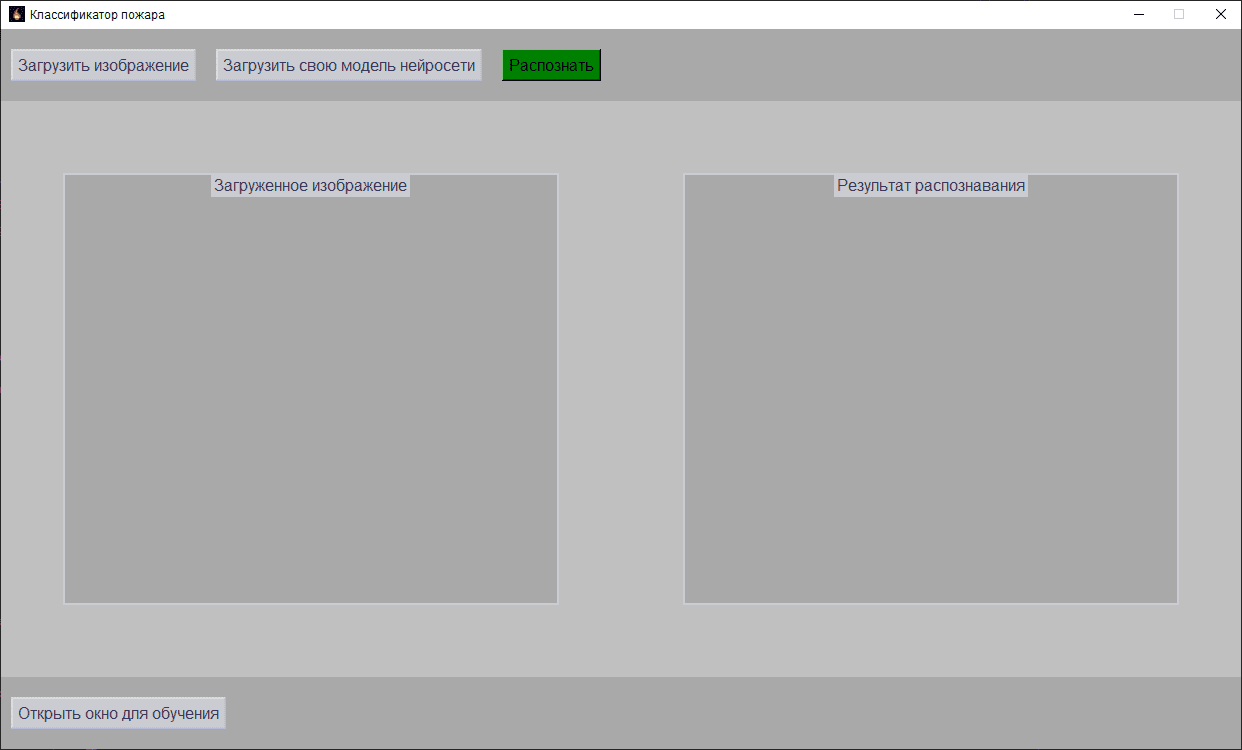
\includegraphics[width=1\linewidth]{systemtest1}
\caption{Интерфейс программы. Основное окно}
\label{systemtest1:image}
\end{figure}

\begin{figure}[H]
\centering
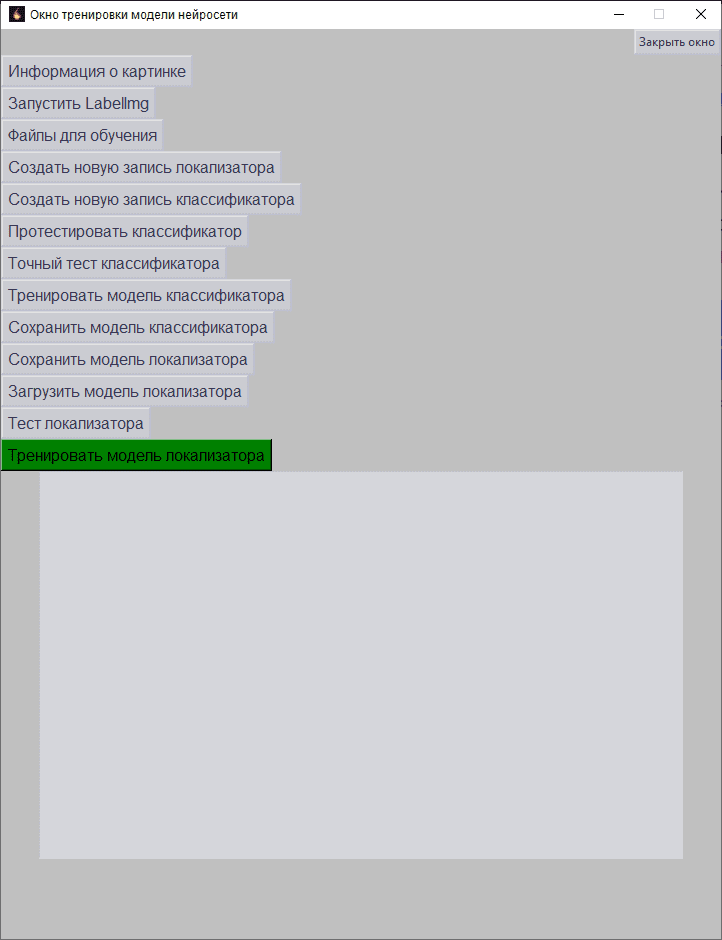
\includegraphics[width=1\linewidth]{systemtest13}
\caption{Интерфейс программы. Окно обучения.}
\label{systemtest13:image}
\end{figure}

На рисунке \ref{systemtest2:image} предоставлен вариант с загрузкой изображения.

\begin{figure}[H]
\centering
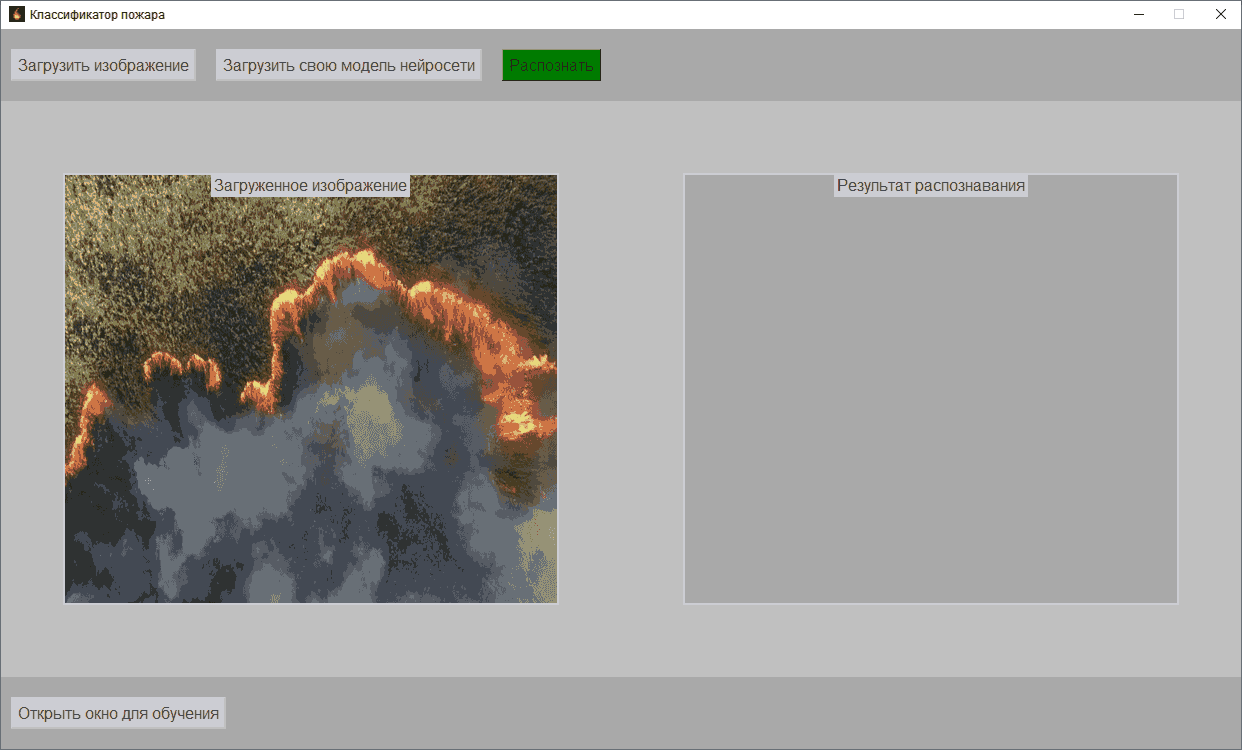
\includegraphics[width=1\linewidth]{systemtest2}
\caption{Интерфейс программы с загруженным изображением.}
\label{systemtest2:image}
\end{figure}

На рисунке \ref{systemtest4:image} предоставлен вариант с загрузкой пользовательской моделью нейронной сети. Здесь пользователь выбирает путь до файла с весами формата .keras.

\begin{figure}[H]
\centering
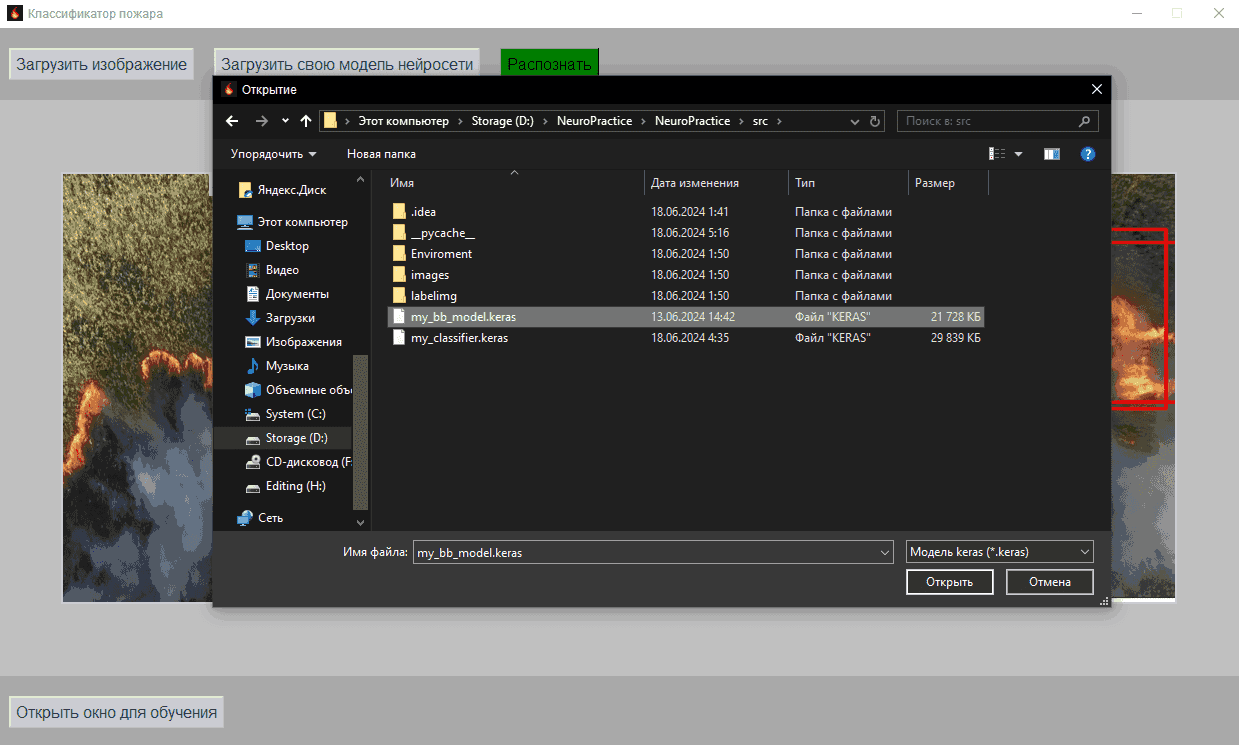
\includegraphics[width=1\linewidth]{systemtest4}
\caption{Функция загрузки пользовательских весов. Выбор файла в диалоговом окне}
\label{systemtest4:image}
\end{figure}

На рисунках \ref{systemtest3:image}-\ref{systemtest12:image} представлены варианты распознования возгораний на изображениях.

\begin{figure}[H]
\center{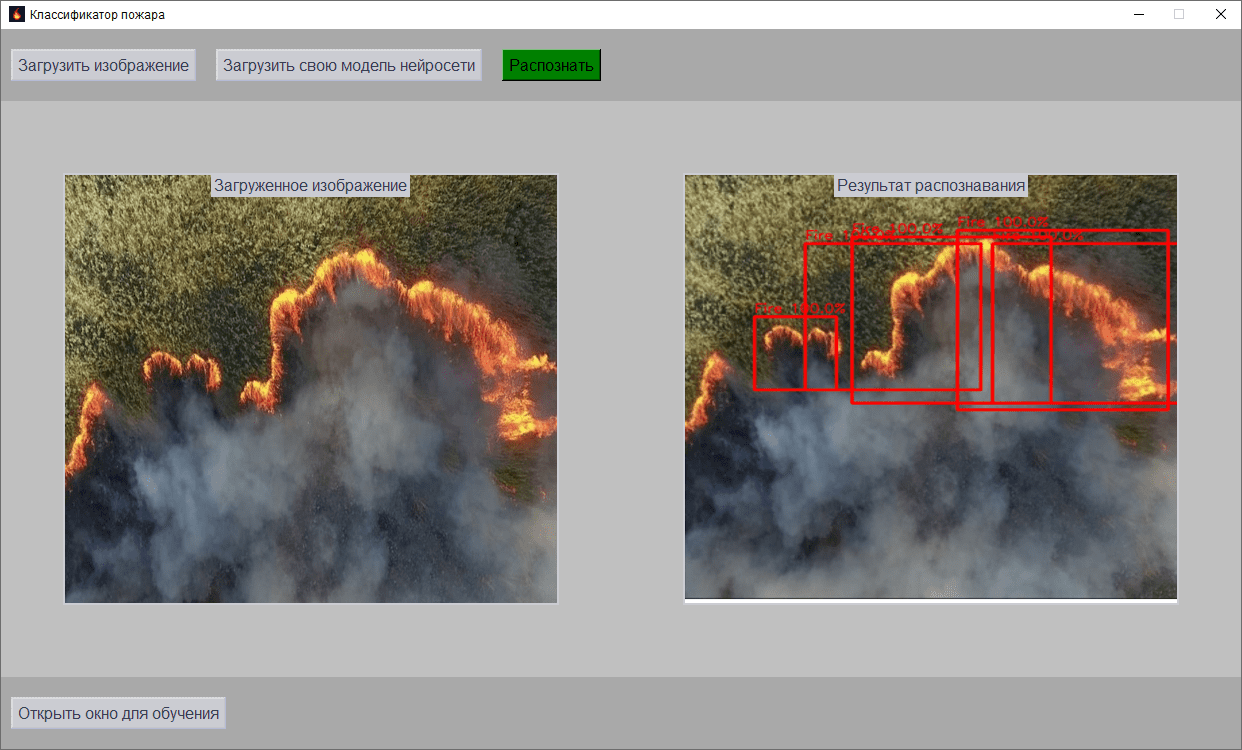
\includegraphics[width=1\linewidth]{systemtest3}}
\caption{Интерфейс с распознанным файлом fire1.png}
\label{systemtest3:image}
\end{figure}

\begin{figure}[H]
\center{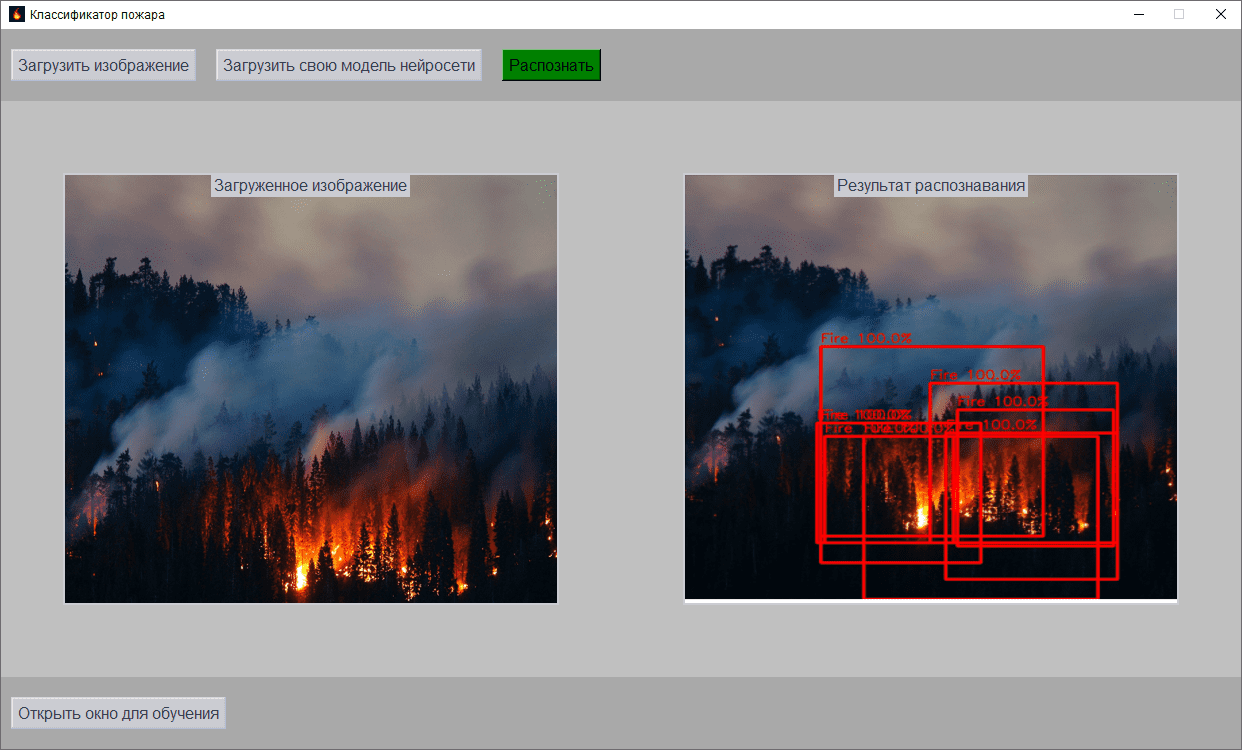
\includegraphics[width=1\linewidth]{systemtest5}}
\caption{Интерфейс с распознанным файлом fire2.png}
\label{systemtest5:image}
\end{figure}

\begin{figure}[H]
\center{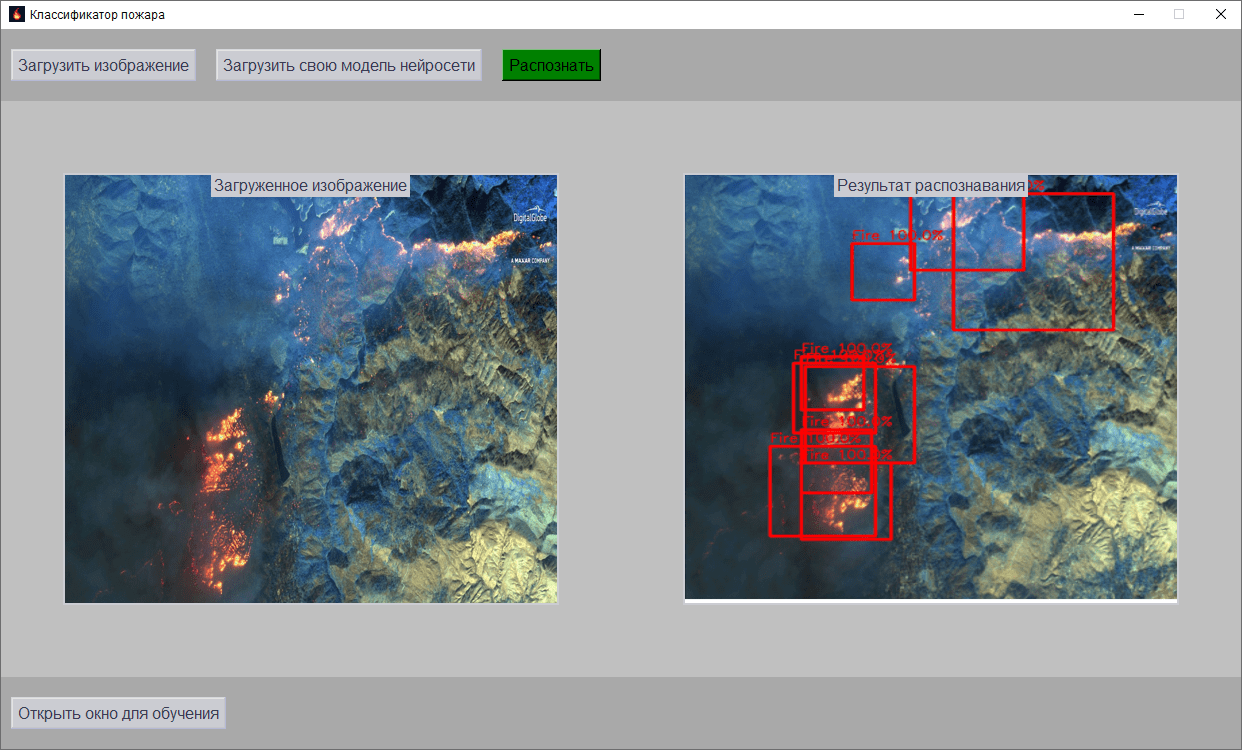
\includegraphics[width=1\linewidth]{systemtest6}}
\caption{Интерфейс с распознанным файлом fire3.png}
\label{systemtest6:image}
\end{figure}

\begin{figure}[H]
\center{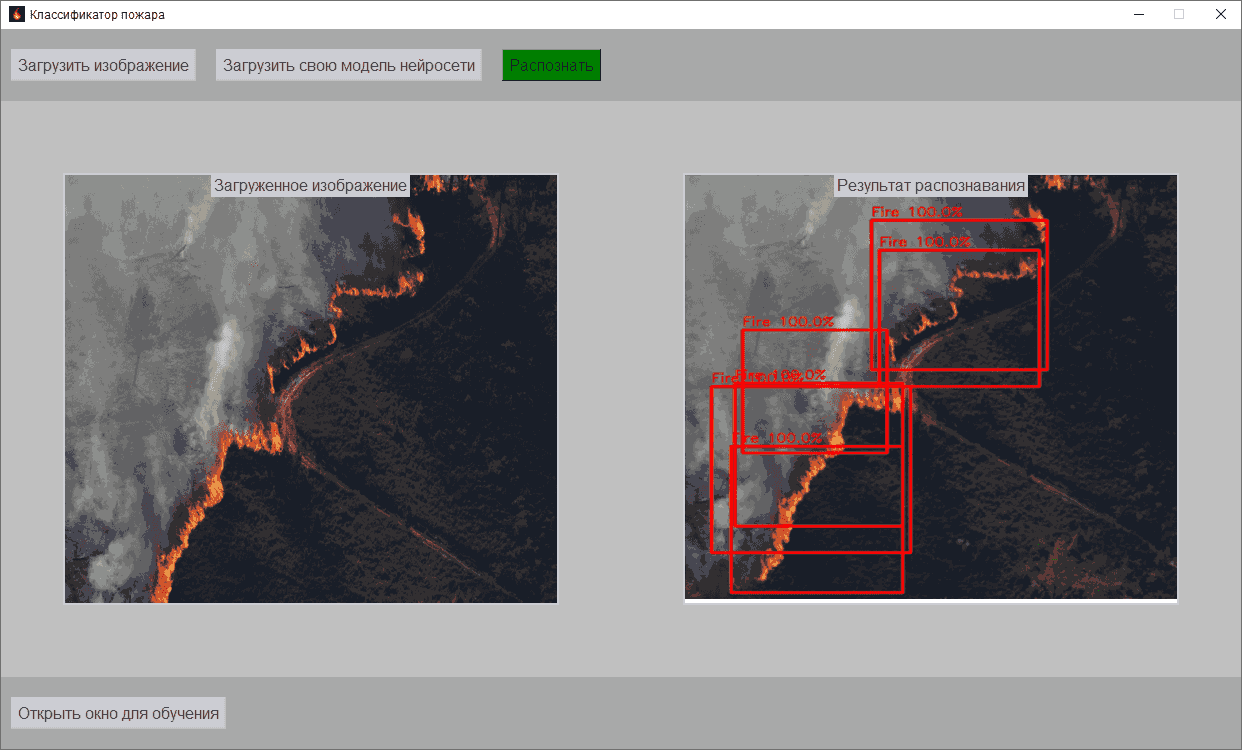
\includegraphics[width=1\linewidth]{systemtest7}}
\caption{Интерфейс с распознанным файлом fire4.png}
\label{systemtest7:image}
\end{figure}

\begin{figure}[H]
\center{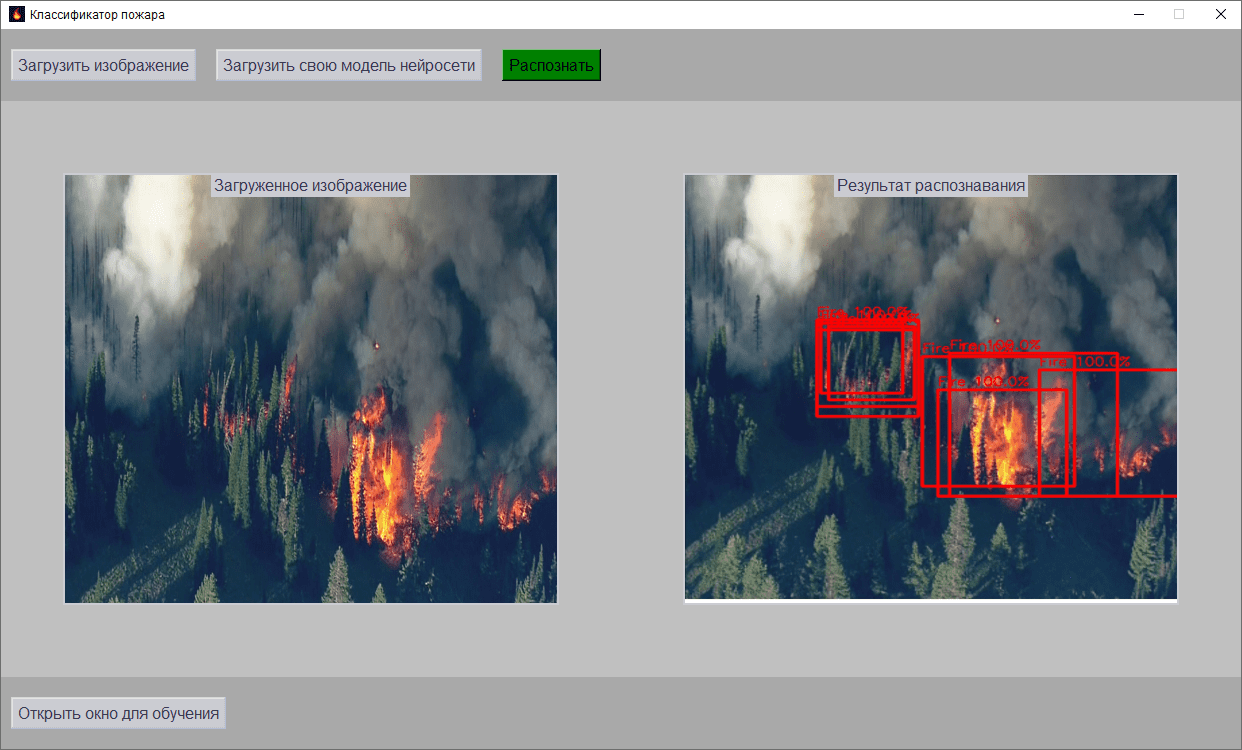
\includegraphics[width=1\linewidth]{systemtest8}}
\caption{Интерфейс с распознанным файлом fire5.png}
\label{systemtest8:image}
\end{figure}

\begin{figure}[H]
\center{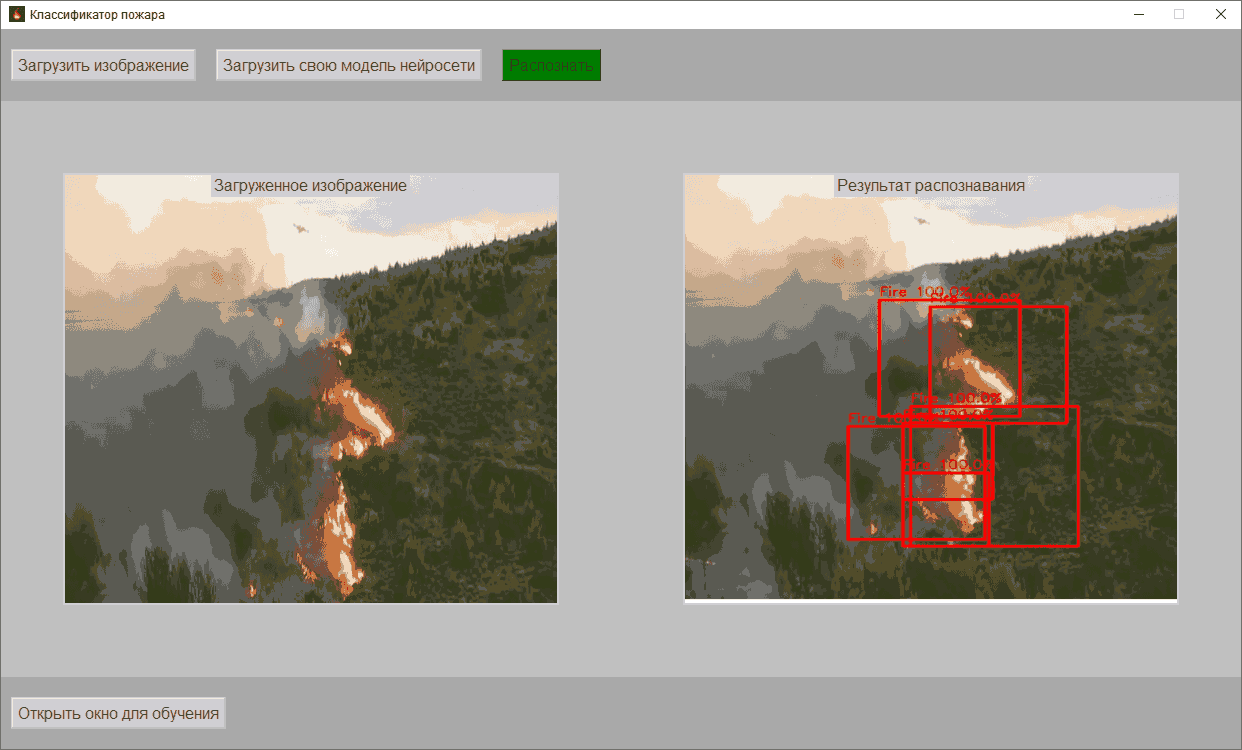
\includegraphics[width=1\linewidth]{systemtest9}}
\caption{Интерфейс с распознанным файлом fire6.png}
\label{systemtest9:image}
\end{figure}

\begin{figure}[H]
\center{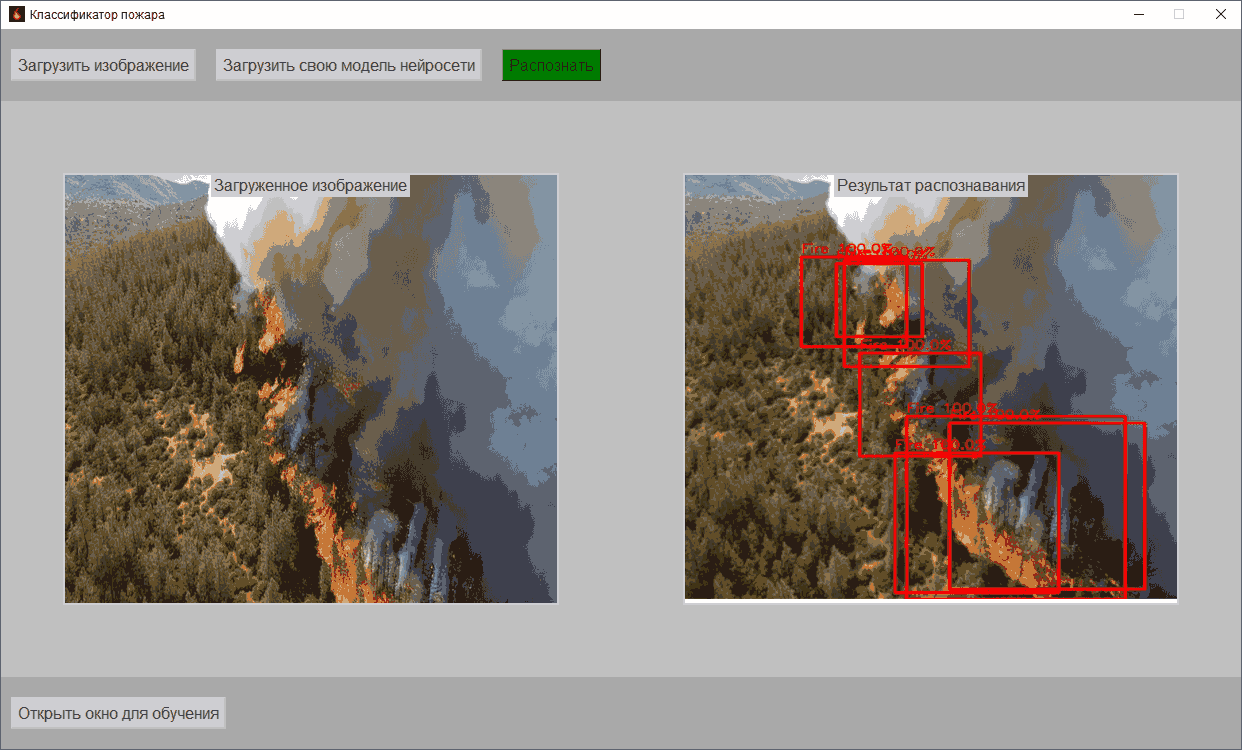
\includegraphics[width=1\linewidth]{systemtest10}}
\caption{Интерфейс с распознанным файлом fire7.png}
\label{systemtest10:image}
\end{figure}

\begin{figure}[H]
\center{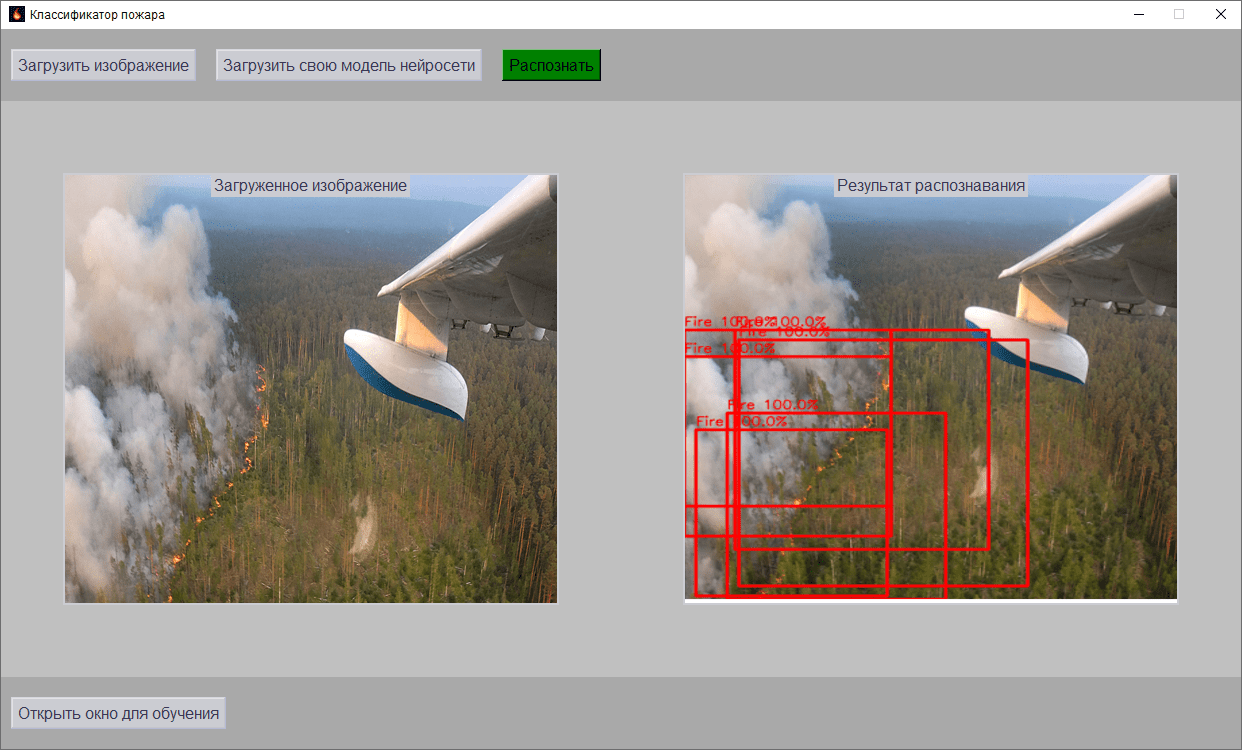
\includegraphics[width=1\linewidth]{systemtest11}}
\caption{Интерфейс с распознанным файлом fire8.png}
\label{systemtest11:image}
\end{figure}

\begin{figure}[H]
\center{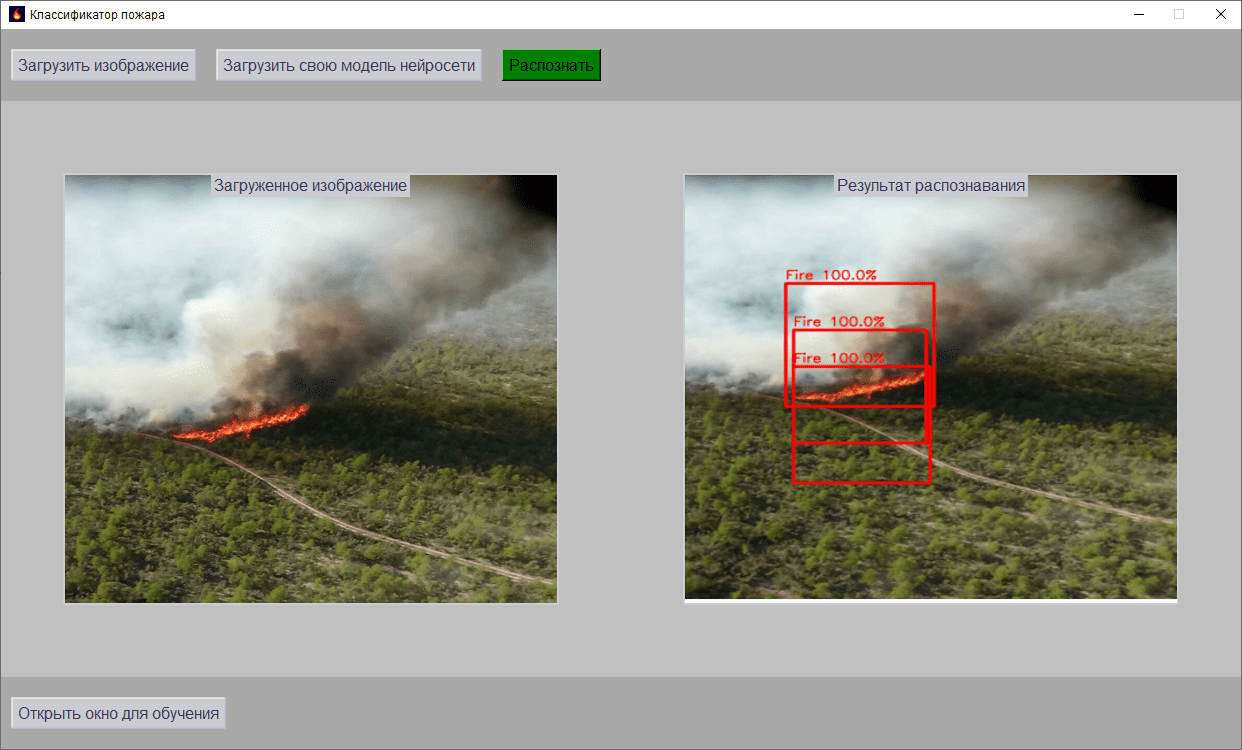
\includegraphics[width=1\linewidth]{systemtest12}}
\caption{Интерфейс с распознанным файлом fire9.png}
\label{systemtest12:image}
\end{figure}

На рисунке \ref{systemtest22:image} была нажата кнопка Информация о картинке, после чего открылось окно с картинкой и вывелась информация по ней.

\begin{figure}[H]
\center{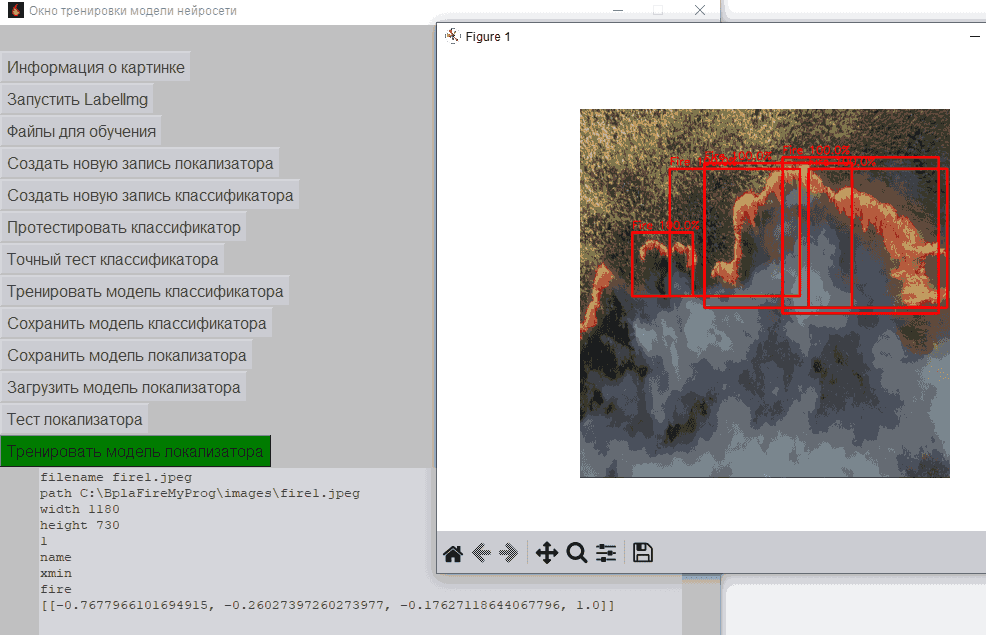
\includegraphics[width=1\linewidth]{systemtest22}}
\caption{Интерфейс дополнительного окна с информацией о картинке и сама картинка}
\label{systemtest22:image}
\end{figure}

На рисунке \ref{systemtest14:image} была нажата кнопка Файлы для обучения, после чего в поле вывода отобразились все файлы, доступные для обучения.

\begin{figure}[H]
\center{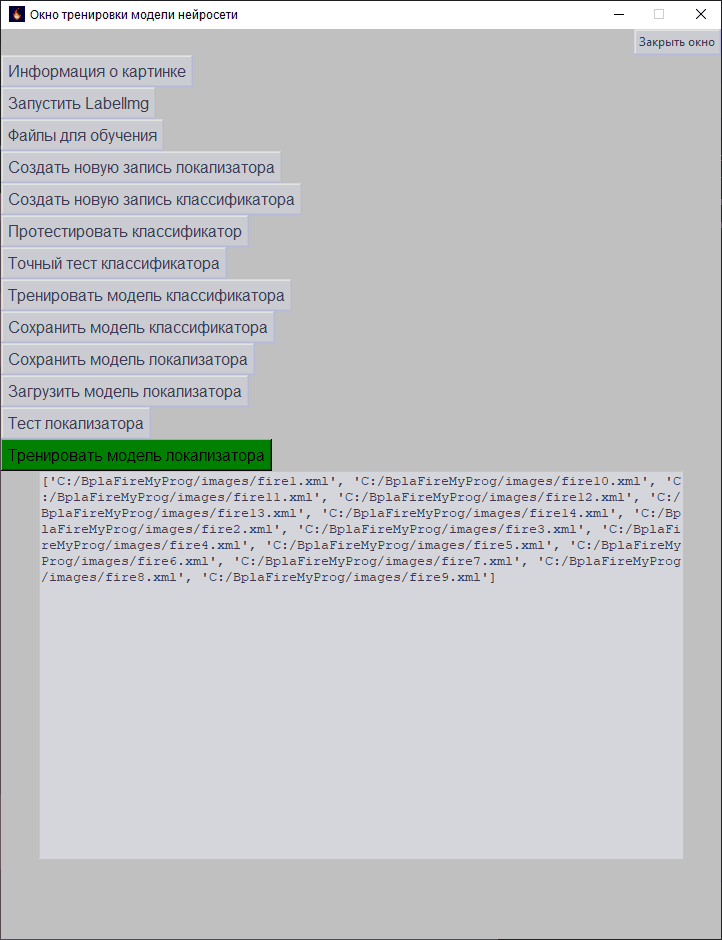
\includegraphics[width=1\linewidth]{systemtest14}}
\caption{Интерфейс дополнительного окна с информацией файлах для обучения}
\label{systemtest14:image}
\end{figure}

На рисунке \ref{systemtest15:image} была нажата кнопка Протестировать классификатор, после чего открылось новое окно, где показаны обрезанные фрагменты изображений, которые сеть классифицировала (0 - нет возгорания, 1 - есть возгорание).

\begin{figure}[H]
\center{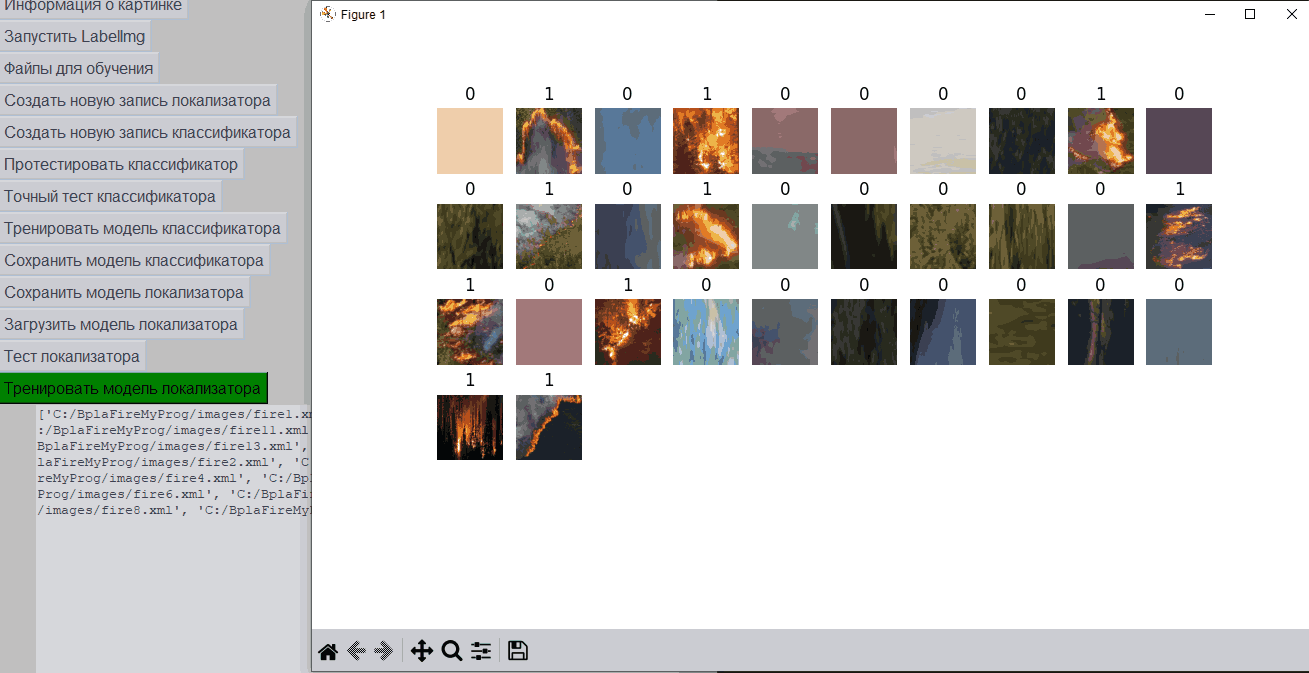
\includegraphics[width=1\linewidth]{systemtest15}}
\caption{Интерфейс дополнительного окна и окно с классификацией фрагментов изображений}
\label{systemtest15:image}
\end{figure}

На рисунке \ref{systemtest16:image} была нажата кнопка Точный тест классификатора, после чего открылось новое окно, где показаны обрезанные фрагменты изображений, которые сеть классифицировала и придала степень принадежности с уровнем ошибки.

\begin{figure}[H]
\center{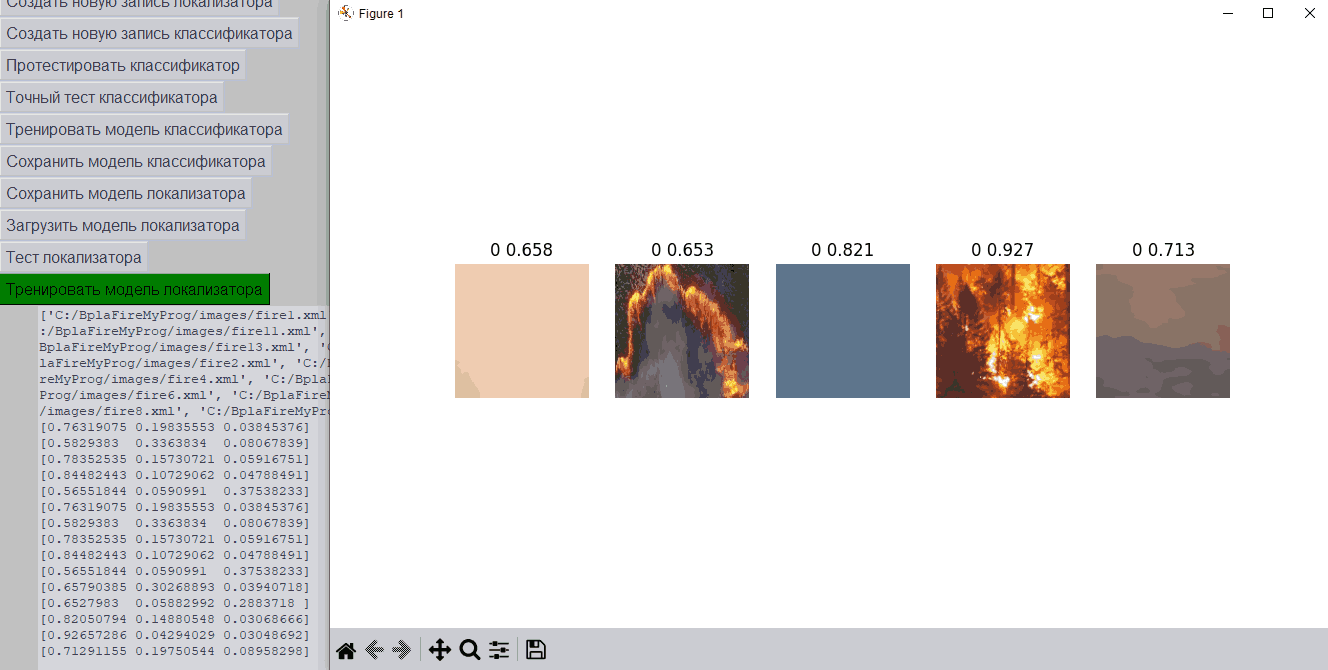
\includegraphics[width=1\linewidth]{systemtest16}}
\caption{Интерфейс дополнительного окна и окно с классификацией фрагментов изображений и уровнем ошибки}
\label{systemtest16:image}
\end{figure}

На рисунке \ref{systemtest17:image} была нажата кнопка Тренировать модель классификатора, после чего открылось новое окно с диаграммой, где наглядно видно, как функция стремится к 0, тем самым показывая точность распознования классификатора.

\begin{figure}[H]
\center{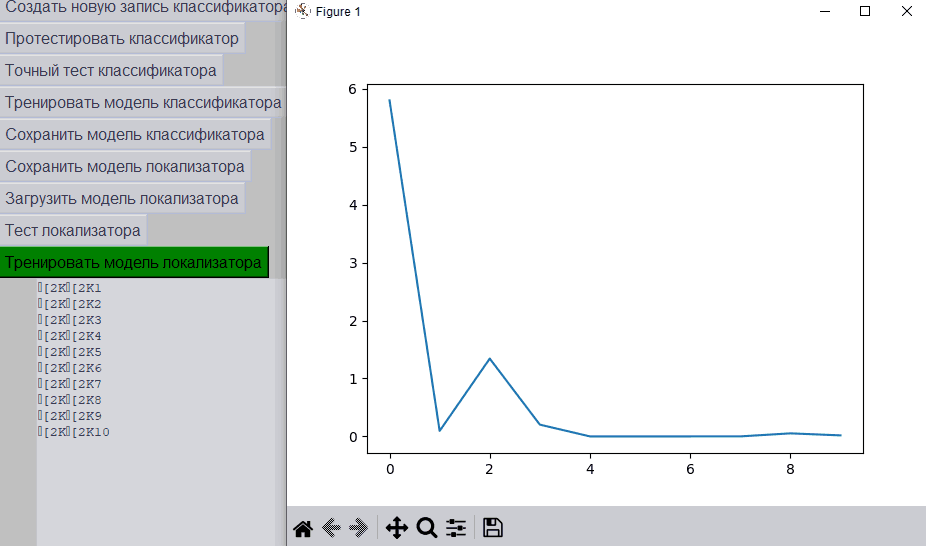
\includegraphics[width=1\linewidth]{systemtest17}}
\caption{Интерфейс дополнительного окна и окно с диаграммой уровня ошибки нейросети классификатора}
\label{systemtest17:image}
\end{figure}

На рисунке \ref{systemtest18:image} была нажата кнопка Тест локализатора, но не была загружена модель НС локализатора, после чего изображения были распознанны некорректно.

\begin{figure}[H]
\center{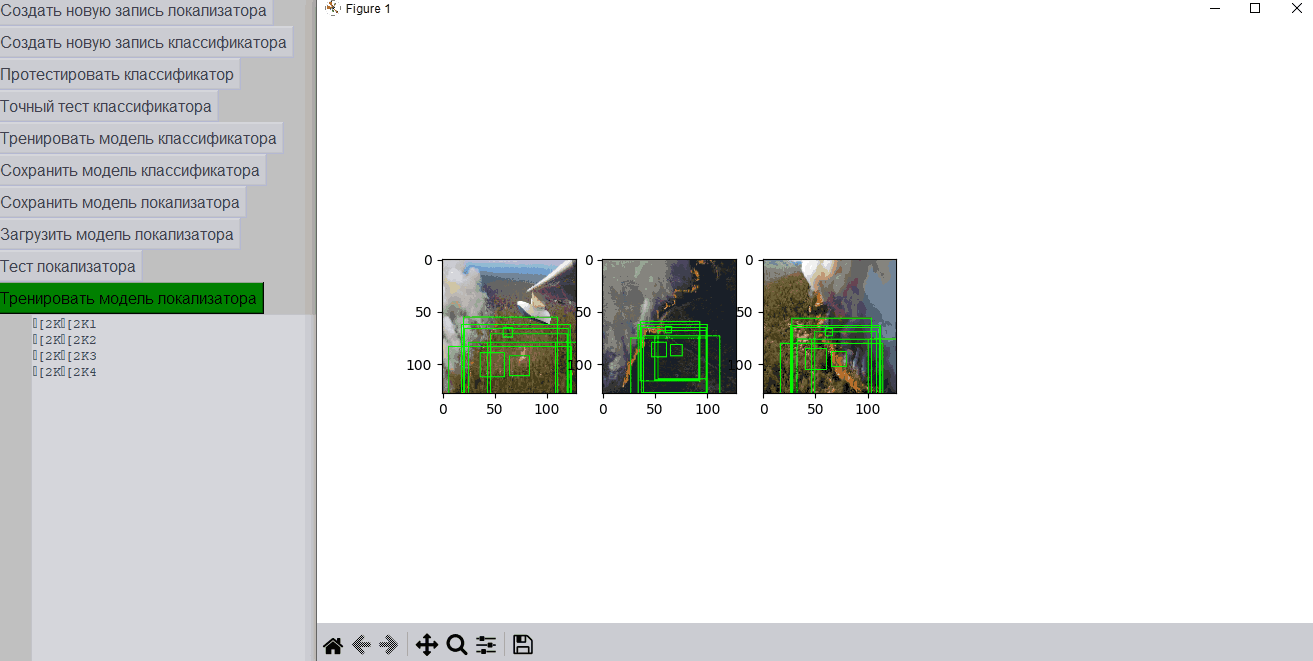
\includegraphics[width=1\linewidth]{systemtest18}}
\caption{Интерфейс дополнительного окна и окно с некорректно распознанными изображениями}
\label{systemtest18:image}
\end{figure}

На рисунке \ref{systemtest19:image} была нажата кнопка Тест локализатора и была загружена модель НС локализатора, после чего изображения были распознанны корректно.

\begin{figure}[H]
\center{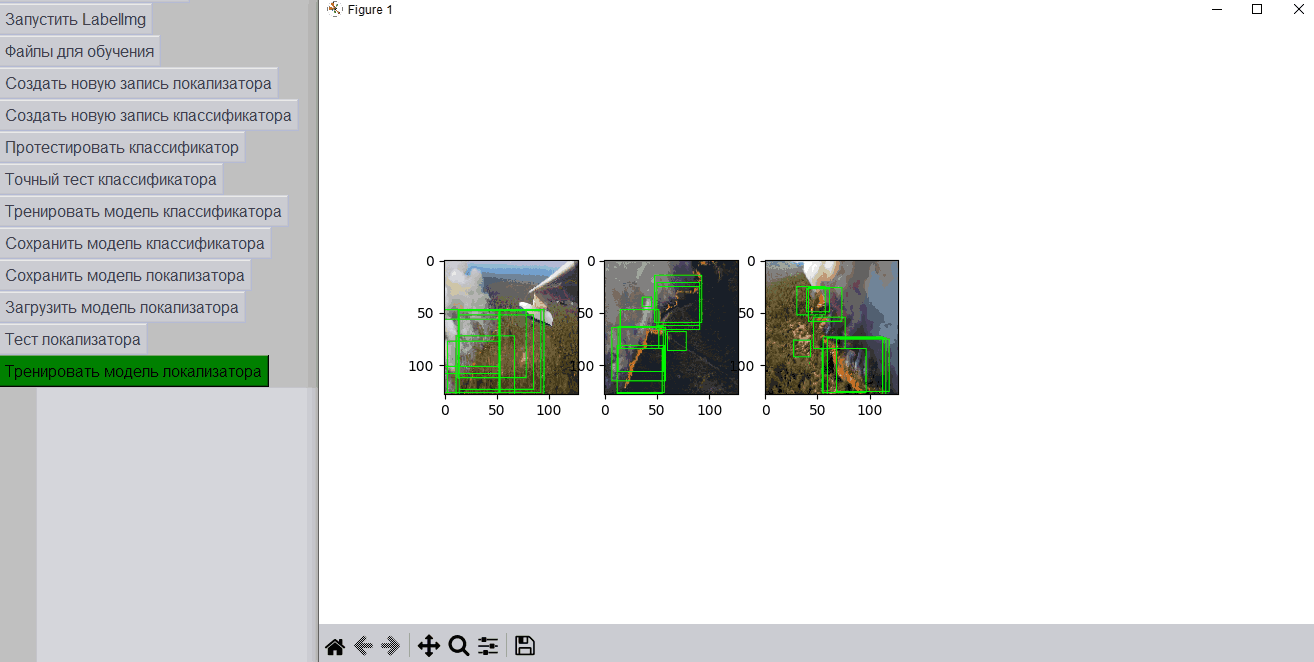
\includegraphics[width=1\linewidth]{systemtest19}}
\caption{Интерфейс дополнительного окна и окно с корректно распознанными изображениями}
\label{systemtest19:image}
\end{figure}

На рисунках \ref{systemtest20:image} - \ref{systemtest21:image}  была нажата кнопка Тренировать модель локализатора и была загружена модель НС локализатора, после чего, спустя несколько эпох, изображения были распознанны. На диаграмме можно наглядно увидеть, что значения близки к 0 и даже выходят за абстрактные значения в минус.

\begin{figure}[H]
\center{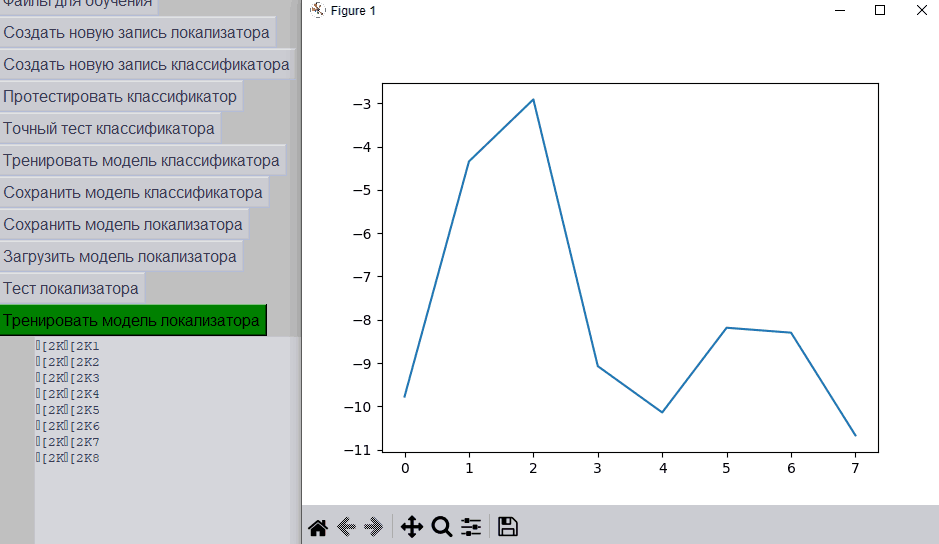
\includegraphics[width=1\linewidth]{systemtest20}}
\caption{Интерфейс дополнительного окна и окно с диаграммой ошибки локализатора}
\label{systemtest20:image}
\end{figure}

\begin{figure}[H]
\center{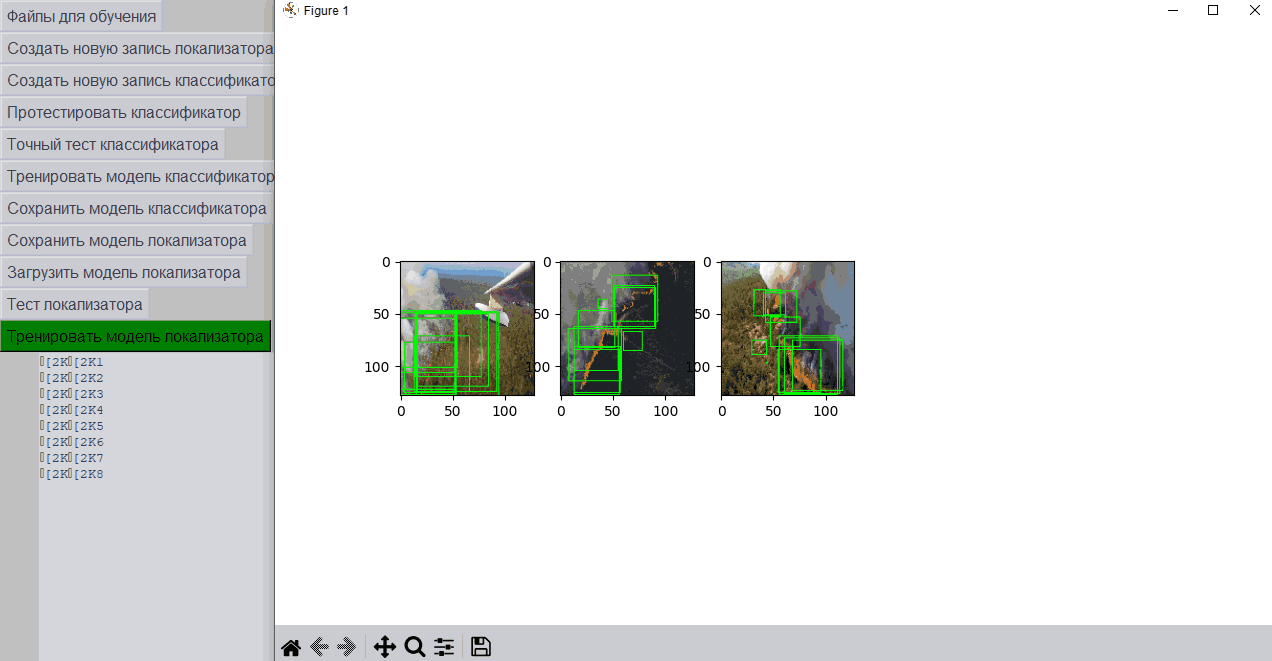
\includegraphics[width=1\linewidth]{systemtest21}}
\caption{Интерфейс дополнительного окна и окно с распознанными изображениями после нескольких эпох}
\label{systemtest21:image}
\end{figure}

На рисунках \ref{systemtestlabelimg2:image} - \ref{systemtestlabelimg1:image}  была нажата кнопка Запустить LabelImg, после чего появилось окно с предупреждением о необходимости дополнительных пакетов. После подтвердждения открылось окно со сторонним приложением, которое поможет выделить объекты на изображениях для дальнейшего сохранения их данных в формате xml.

\begin{figure}[H]
\center{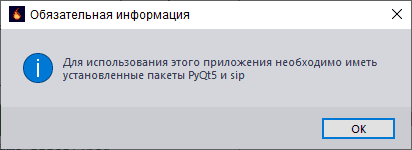
\includegraphics[width=1\linewidth]{systemtestlabelimg2}}
\caption{Интерфейс дополнительного окна и окно с распознанными изображениями после нескольких эпох}
\label{systemtestlabelimg2:image}
\end{figure}

\begin{figure}[H]
\center{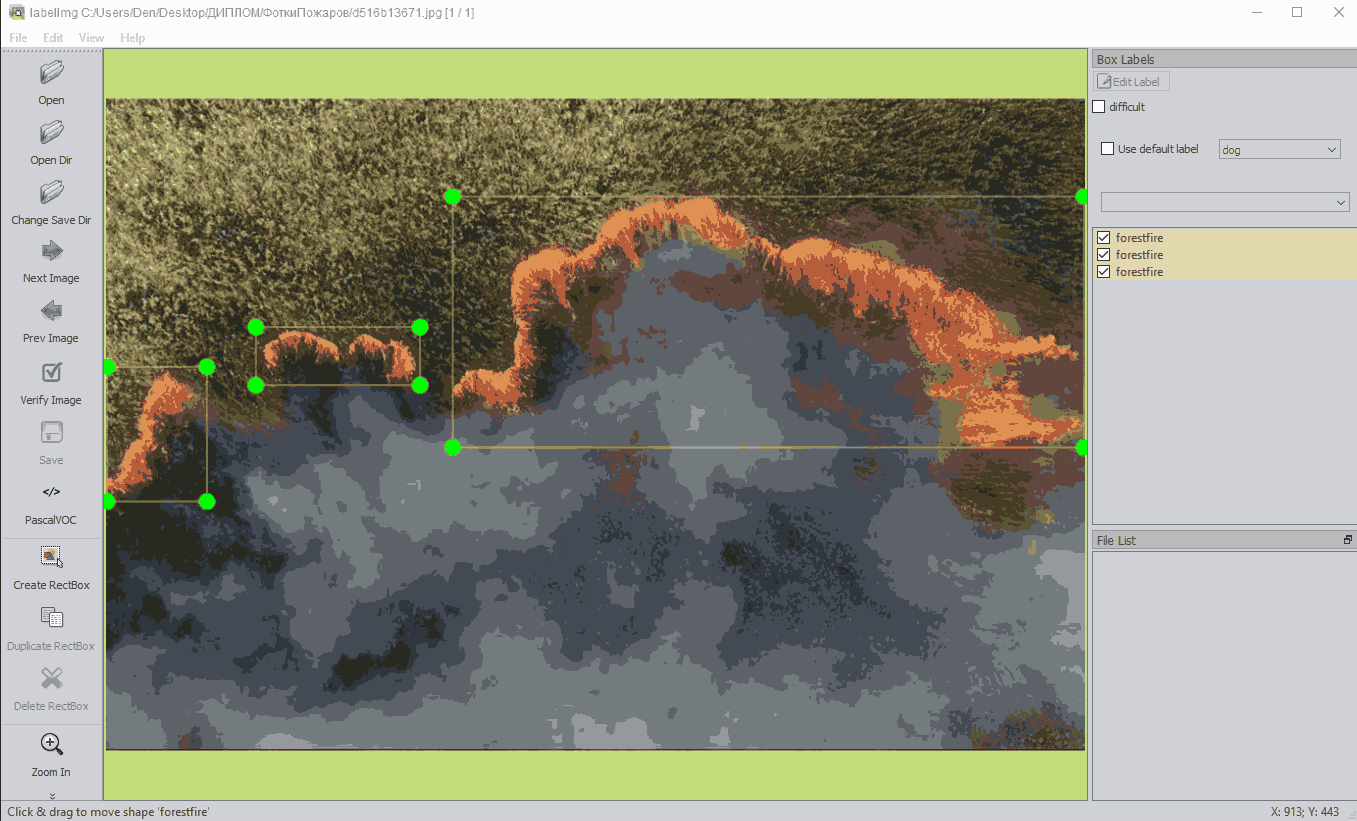
\includegraphics[width=1\linewidth]{systemtestlabelimg1}}
\caption{Интерфейс дополнительного окна и окно с распознанными изображениями после нескольких эпох}
\label{systemtestlabelimg1:image}
\end{figure}
